\documentclass[twoside]{mfa}

%%%% Please do not edit this part %%%%%%%%%%%%%%%%%%%%%%%%%%%%%%%%%%%%%%%%%%%%%%%%%%%%%%%%%%%%%%%%%%%%%%%%%%
%\usepackage{geometry}
%\geometry{paperheight=25cm,paperwidth=17.6cm,inner=25.5mm,top=32mm,textwidth=12.5cm,textheight=19.7cm}
\usepackage{amssymb,amsfonts}
\renewcommand\volume{{\bf 8} (2021)}        %% volume
%\setcounter{page}{3}
%%%%%%%%%%%%%%%%%%%%%%%%%%%%%%%%%%%%%%%%%%%%%%%%%%%%%%%%%%%%%%%%%%%%%%%%%%%%%%

%%% Additional packages %%%%%%%%%%%%%%%%%%%%%%%%%%%%%%%%%%%%%%%%%%%%%%%%%%%%%%%%%%%%%%%%%%%%%%%%%%%
\usepackage{graphicx}
\usepackage{float}


%%%%%%%% User's macros %%%%%%%%%%%%%%%%%%%%%%%%%%%%%%%%%%%%%%%%%%%%%%%%%%%%%%%%%%%%%%
\newcommand\refrm[1]{{\rm (\ref{#1})}}
\newcommand\bbreak{\allowdisplaybreaks}
\newcommand\dd{\mathop{\rm d\!}\nolimits}
\newcommand\sgn{\mathop{\rm sgn}\nolimits}
\newcommand\dx[1]{\mathrm{d}#1}

\setlength\parindent{0pt}
%%%%%%%%%%%%%%%%%%%%%%%%%%%%%%%%%%%%%%%%%%%%%%%%%%%%%%%%%%%%%%%%%%%%%%%%%%%%%%
\begin{document}
%%============================================================================%%
%%                              title page                                    %%
%%============================================================================%%

\title[Policing Fairness]{Assessing Fair Policing in Austin, TX}

\author[Wu]{Qiuyi Wu$^\ast$}
\address{Department of Biostatistics and Computational Biology,  University of Rochester}
\email{Qiuyi\_Wu@URMC.Rochester.edu}
%\curraddr{}
%\urladdress{http://www.anonymous.com/anonymous/index.html}

\author[Skrill]{David Skrill$^\ast$}
\address{Department of Biostatistics and Computational Biology,  University of Rochester}
\email{David\_Skrill@URMC.Rochester.edu}

\author[Pham]{Cuong Pham}
\address{Department of Biostatistics and Computational Biology,  University of Rochester}
\email{Cuong\_Pham@URMC.Rochester.edu}


%\dedicatory{Dedicated to ...}
\thanks{The research was part of data analytics competition in 2021 Upstat Annual Conference, and was supported by The American Statistical Association, and RIT Department of Criminal Justice, Fox Pest Control – Rochester, and Wegmans. \\ 
$^\ast$ These authors contributed equally to this work}

%%%%%%%% Keywords %%%%%%%%%%%%%%%%%%%%%%%%%%%%%%%
\keywords{Fairness, policing, traffic stops, racial disparities}

%%%%%%%% AMS classification 2010 %%%%%%%%%%%%%%%%%%%%%%%%
%\subjclass{34K06, 34K25}{39}      %% \subjclass{primary}{secondary}

%%%%%%%% Abstract %%%%%%%%%%%%%%%%%%%%%%%%%%%%%%%%%%%%
\begin{abstract}
This report demonstrates disparities by race in traffic stops by the Austin Police Department. After
exploratory analysis, we assess various models and statistics derived from the hit rate and using the Veil
of Darkness. We conclude with a Bayesian hierarchical model that produces officer-level posteriors for the
hit rate.
\end{abstract}

%%%%%%%% Environments Theorem, Definition, etc. %%%%%%%%%%%%%%%%%%%%%%%%%%%%%%%%%%%
\newtheorem{theorem}{Theorem}[section]
\newtheorem{corollary}[theorem]{Corollary}
\newtheorem{lemma}[theorem]{Lemma}
\newtheorem{proposition}[theorem]{Proposition}

\theoremstyle{definition}
\newtheorem{definition}[theorem]{Definition}
\newtheorem{problem}[theorem]{Problem}
\newtheorem{example}[theorem]{Example}
\newtheorem{remark}[theorem]{Remark}

%\theoremstyle{remark}
%\newtheorem{remark}[theorem]{Remark}

\numberwithin{equation}{section}

%%%%%%% Ttitlepage typesetting %%%%%%%%%%%%%%%%%%%%%%%%%%%%%%%%%%%%%%%%%
\maketitle

%%======================================================================%%
%%                             Article body                             %%
%%======================================================================%%
\section{Introduction}
This paper investigates racial disparities in traffic stops by the Austin Police Department. Using data available from Austin Open Data, a Texas government-run data portal, and from the Stanford Open Policing Project, we evaluate these disparities using models derived from the “hit rate” and the effect of the “veil of darkness”, two often-cited methods for assessing fair policing. Our main report consists of three parts. First, we conduct an exploratory data analysis to get a big picture of policing in Austin. Second, we use various modeling strategies to assess the severity of racial disparities. Third, we propose a measure of fairness based on the differences in the posterior median hit rate among individual police officers.



\section{Available Data}
The primary data set is from the Stanford Open Policing Project \footnote{Stanford Open Policing Project (OPP): https://openpolicing.stanford.edu/data/} (from here on referred to as the Stanford data). This data set record stops made by Austin Police Department (APD) over a roughly ten year period (2006.01.01 - 2016.06.30) and contains information such as the date of stops, subject’s race, whether the subject was searched or frisked, and whether any contraband were found. Notably, this data lacks information about the time or place of the stops. Because the 2016 data is incomplete, we focus on the data for which we have complete years (2006-2015) for the first two prats of the analysis; this contains 463,944 stops.  We note that the distribution of stops per officer has an extremely long tail.\\

We also make use of data from the 2019 Racial Profiling report, available from Austin Open Data (and
hereafter referred to as the RP data). This data set contains similar information as the Stanford data, with
additional information about the event time, location, and officer race. Notably, the race of the subject is
missing from this data.\\

Lastly, we use US census demographic data. Specifically, we use 2017 5-year American Community Survey
zip-code-level data with the Stanford data, and 2019 census population data for 2019 Austin RP data. In
addition, we also refer to the racial profiling reports published the Austin Police Department.


\section{Exploratory Analysis}

We first examine the count of stops by race during 2006-2015 (Table \ref{tb:1}), using the Stanford Data. It is notable that over half of the stops involved were of white subjects, about four times the number of stops of Black people. According to 5-year census data, the white population in Austin (445,269) is almost 7 times than the black population (66,724). Examining figure \ref{fg:1}, we can see that at least for Black, Hispanic and white drivers, the annual trends are very different by race.\\

We see that the proportion of stops of white people declined from the beginning of the study period to the end, whereas the proportion of stops of Hispanic and Black people rose and remained roughly constant, respectively.  

\begin{table}
\centering
\begin{tabular}{l*{3}{c}} 
\hline
Driver Race & Counts & Proportion \\
\hline
asian/pacific & 11658 & 0.033  \\
black & 52381 & 0.147\\
hispanic & 765707 & 0.215\\
other & 2105 & 0.006\\
unknown & 2622 & 0.007\\
white & 211588 & 0.593\\
\hline
\end{tabular}
\caption{Proportion of stops by race during 2006-2015} \label{tb:1}
\end{table}

\begin{figure}[H]
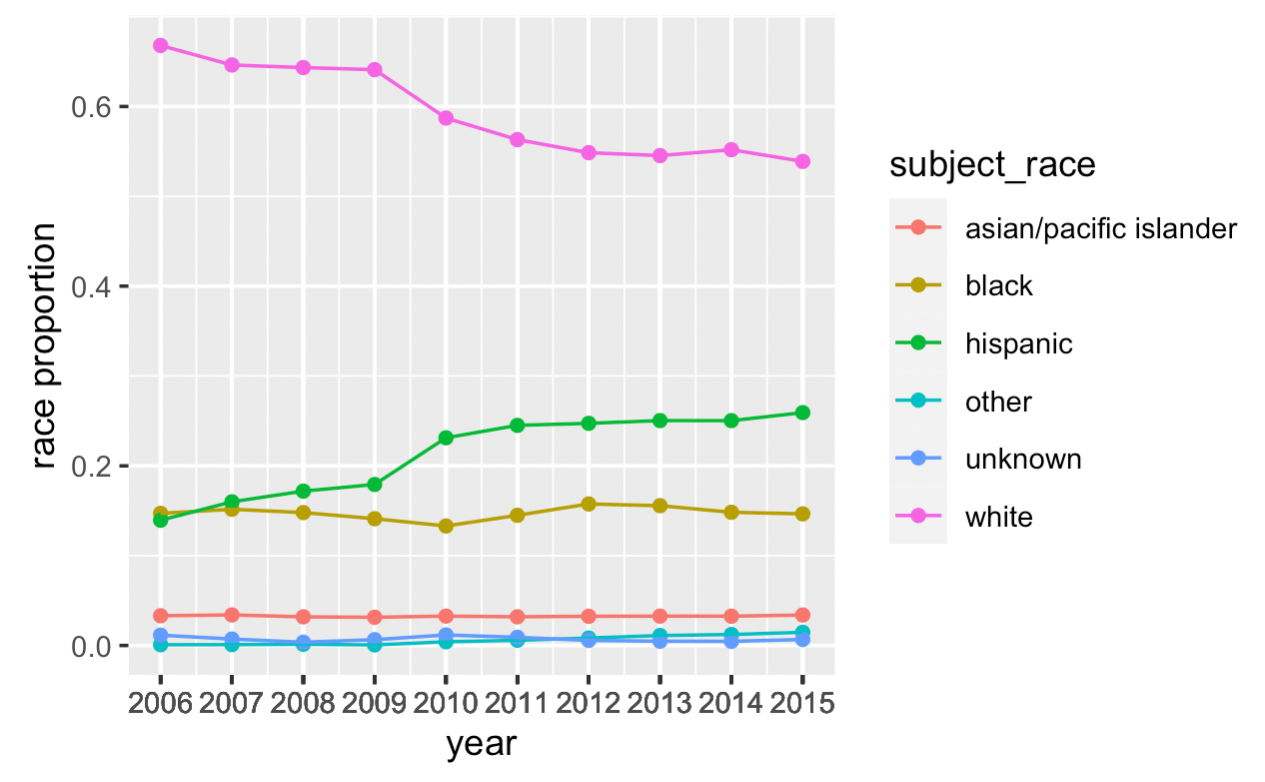
\includegraphics[width=10cm]{pic1.png}
\caption{Race proportion in each year} \label{fg:1}
\end{figure}


\subsection{Benchmark Test}
As mentioned previously, the number of the white drivers stopped is four times of the black drivers, while the white population in Austin is actually over 6 times of the black population. We define the *stop rate* for a given race as follows.  
\begin{align*}
\text{Stop Rate}_i = \frac{\text{Number of Stops for Race }i}{\text{Population of Race }i}
\end{align*}

From Table \ref{tb:2}, we can see black drivers are stopped with a rate much higher than the drivers of other races. We can investigate this further by looking at other benchmarks such as search rate and frisk rate with stopped population as baseline.

\begin{align*}
\text{Search Rate}_i = \frac{\text{Number of Stopped People Who Were Searched for Race }i}{\text{Number of Stops for Race }i}
\end{align*}

\begin{align*}
\text{Stop Rate}_i = \frac{\text{Number of Stopped People Who Were Frisked for Race }i}{\text{Number of Stops for Race }i}
\end{align*}


Again, from the last two columns of Table \ref{tb:2}, we can see Black and Hispanic drivers are searched with a rate 3 times higher than white drivers, and almost 8 times higher than Asian/Pacific drivers. The Black and Hispanic drivers are also frisked at a rate much higher than the drivers of other races.\\



\begin{table}
\centering
\begin{tabular}{l*{9}{c}} 
\hline
Driver Race & Counts& Population &Proportion &Stop Rate& Search Rate& Frisk Rate& Hit Rate \\
\hline
asian/pacific& 11658 &63752 &0.033& 0.183 &0.015 &0.011& 0.188\\
black &52381 &66724 &0.147 &0.785 &0.092   &0.039 &0.254\\
hispanic &765707 &316709 &0.215 &0.242   & 0.086 &0.044 &0.323\\
white &211588 &445269 &0.593    &0.475   & 0.031 &0.021& 0.318\\
\hline
\end{tabular}
\caption{Stop rates, search rates and frisk rates during 2015} \label{tb:2}
\end{table}



The racial disparity by the police is clear from benchmark test, but it is insufficient evidence of discriminative policing. Athough this is strong evidence that stopped non-white drivers are searched and/or frisked at a higher rate than stopped white drivers, it is insufficient for making claims about the presence of discriminatory policing practices. We need to check if different race groups are disproportionately stopped corresponding to their rates of violating the law.





\subsection{Outcome Test}

In order to access this, we shall look at the result of searches to see at what rate searched drivers are found to be doing something illegal. Here, we define a successful search as one that uncovers contraband, and we define the hit rate as the proportion of searches that are successful.

\begin{align*}
\text{Hit Rate}_i = \frac{\text{Number of Contraband Uncovered for Race }i}{\text{Number of Searched People for Race }i}
\end{align*}

If racial groups have different hit rates, it can be taken as evidence of discriminative policing: if the hit rate for group i is lower than the hit rate for group j, it may be the case that there is a lower evidenciary standard used when deciding whether to search or frisk a person belong to group i relative to that for a person belonging to group j. From the last column in Table \ref{tb:2}, we can see the hit rate for Black and Asian/Pacific drivers are lower than for white and Hispanic drivers, indicating police may have a lower threshold of evidence when searching Black or Asian/Pacific drivers.


\subsection{Veil of Darkness Test \& Fisher’s Exact Test}

According to Grogger and Ridgeway, the “Veil of Darkness” test can help assess the bias in the stop decisions. The hypothesis of this test states that officers who are engaged in racial profiling are less likely to be able to identify a driver’s race after dark than during daylight. Under this hypothesis, if stops made after dark had smaller proportion of black drivers stopped than stops made during daylight, it could be evidence of racial profiling.\\

Because neither of our data sets contain both driver races and stop time information, we propose an indirect way by measuring the racial population in different areas through zip codes by 2019 RP data provided by Austin Police Department. In order to accurately distinguish the daytime and nighttime, we compute the daily subset and dusk time for Austin in 2019. In Table \ref{tb:3} we can see earliest sunset in 2019 was at around 17:32 in early December and it goes fully dark in 26 minutes. The latest sunset time was around 20:38 late June and it was fully dark after 28 minutes.\\

\begin{table}
\centering
\begin{tabular}{l*{9}{c}} 
\hline
Date &Sunset &Dusk &Sunset Minute& Dusk Minute \\
\hline
2019-12-02 &17:31:42 &17:57:48 &1051 &1077\\
2019-12-01 &17:31:45 &17:57:48 &1051 &1077\\
2019-06-30 &20:37:58 &21:05:27 &1237 &1265\\
2019-06-29 &20:37:56 &21:05:27 &1237 &1265\\
\hline
\end{tabular}
\caption{Minimum and maximum dusk time during the 2019 in Austin} \label{tb:3}
\end{table}


We denote the stops happening before sunset as Daytime Stop, and the stop happening after the dusk as Nighttime Stop. We exclude stops occurring between sunset and dusk in this study. Using zip-code level demographic data, we label zip codes as either a White Majority Area (WMA) or a Black Majority Area (BMA), depending on the demographics of the zip code under consideration. For simplicity of the analysis, we consider only zip codes that have either majority white or majority Black populations.\\


We divide the stops happening in each zip codes into two categories: daytime stops or nighttime stops, and we treat two rows in Table \ref{tb:4} as independent binomial samples. Of $n_1 = 250$ recorded stops in black dominated area, 124 stops happened during the daytime, a proportion of $p_1 = 124/250 = 0.496$. Of $n_2 = 5153$ recorded stops in white dominated area, 2937 stops happened during the daytime, a proportion of $p_2 = 2937/5153 = 0.570$. The sample difference of proportions is 0.074. Using Fisher's exact test to test the null hypothesis of independence of the rows in the following $2 \times 2$ contingency table, we obtain a P-value of 0.02, indicating the strong evidence that the police are not equally likely practicing during day and night to different racial groups.




\begin{table}
\centering
\begin{tabular}{l*{9}{c}} 
\hline
&Day& Night\\
\hline
BMA &124 &126\\
WMA &2937 &2216\\
\hline
\end{tabular}
\caption{Contingency Table} \label{tb:4}
\end{table}



\subsection{Hit Rate and Causal Issues}

In our analysis of observational data, it is important to consider unmeasured confounders. For example, one can argue that it would be unsurprising if more officers patrolled areas with higher crime rates; crime rates are known to be correlated with income and demographic factors. Therefore, if those neighborhoods have higher minority populations, we would expect to see more minority traffic stops. Although this still exposes problems in Austin, it could be interpreted as a problem of economic segregation, not traffic fairness.\\

To overcome this problem, we propose to look at the hit rate with more details in Section 4. We argue that given a person is being searched, the probability of finding contraband items should be equal among all races, regardless of the neighborhood that the search conducted. We want to emphasize that using hit rate does not eliminate all unmeasured confounders, but it helps mitigate the problem.


\section{Modeling}
\subsection{Logistic Regression}

Our descriptive analysis shows that black people in Austin seem to be more likely to be stopped by the police. We are interested in the following question: given a person is stopped, what factors may impact the likelihood of that person being frisked? To investigate this, we fit a logistic regression model with \texttt{frisk} as the dependent variable of \texttt{race}, \texttt{age}, and \texttt{sex}.

$$ \text{Logit}[\Pr(\text{Being Frisked})] = \beta_0 + \beta_1\text{Race} + \beta_2\text{Age} + \beta_3\text{Sex} $$


\begin{table}
\centering
\begin{tabular}{l*{4}{c}} 
\hline
term &estimate &std.error & p.value\\
\hline
(Intercept)  &-2.984 &0.102 &0.000\\
race\_black   &1.503  &0.100  &0.000\\
race\_hispanic& 1.310 &0.099  &0.000\\
race\_white   &0.719 &0.099 & 0.000\\
race\_other   &0.617 &0.180&0.001\\
race\_unknown &0.647 &0.183 &0.000\\
age          &-0.046& 0.001 & 0.000\\
sex\_female   &-1.643 &0.036 & 0.000\\
\hline
\end{tabular}
\caption{Logistic model for frisk rate vs. race, age, and sex} \label{tb:5}
\end{table}



We want to investigate how likely it is that contraband is found, given that a search is performed. This is equivalent to calculating hit rate defined previously. We argue that if racial bias does not exist, the hit rate should be equal for all races. In other words, we expect to find that \texttt{race} is not an essential factor in the model.

$$ \text{Logit}[\Pr(\text{Contraband found})] = \beta_0 + \beta_1\text{Race} $$


\begin{table}
\centering
\begin{tabular}{l*{4}{c}} 
\hline
term &estimate &std.error & p.value\\
\hline
(Intercept)         & -1.988 &0.222 &0.000\\
race\_black   & 0.899 &0.225 & 0.000\\
race\_hispanic& 0.941 &0.224 & 0.000\\
race\_white   & 0.826 &0.224 & 0.000\\
race\_other   & 0.796 &0.355 & 0.025\\
race\_unknown &-0.209 &0.416 & 0.616\\
\hline
\end{tabular}
\caption{Logistic model for contraband found vs. race} \label{tb:6}
\end{table}



We also break down the type of contraband found into three categories: Drugs, Weapons, and Others. We also fit a logistic regression model for each of these categories with \texttt{Race} as the sole independent variable. \\



\begin{table}
\centering
\begin{tabular}{l*{4}{c}} 
\hline
Contraband found &Drugs &Weapons &Others\\
\hline
(Intercept)& -5.24*** (1.00)&-3.61*** (0.45)& -2.38*** (0.26)\\
Black       & 1.10(1.01) &0.32(0.46) &  0.99***(0.26)\\
Hispanic    & 1.21(1.01) &0.36(0.46) & 1.04*** (0.26)\\
White       & 0.73(1.01) &0.98* (0.46)&  0.72** (0.26)\\
Other       & 0.97(1.42) &0.47(0.74) &0.87* (0.40)\\
Unknown   &-11.33(280.85)& 0.04(0.85) &-0.23(0.53)\\
\hline
\end{tabular}
\caption{Contraband Found Break Down (***: $p < 0.001$;
**: $p < 0.01$; *: $p < 0.05$)} \label{tb:7}
\end{table}


From table \ref{tb:5} we see that Black and Hispanic people are more likely to be frisked than white people. The estimated odds of a Black person being frisked are 2.22 time those for a white person. This odd ratio for Hispanic people is 1.8. Asian people are the least likely to be frisked. From table \ref{tb:6} and table \ref{tb:7}, contraband items are more likely to be found for Hispanic and black people. White people are more likely to be found with weapons and Black and Hispanic people are more likely to be found with contraband items that are neither drugs or weapons.



\subsection{Bayesian Modeling}
\subsubsection{Investigating the Hit Rate}

The “hit rate,” defined here as the proportion of times an officer finds contraband given that a frisk has been performed, is a widely-used measure for assessing potentially-discriminatory policing. The hit rate can be thought of as a proxy for “evidence” when an officer decides whether to conduct a search or a frisk; a lower hit rate for a particular segment of the population can signal that an officer has a lower threshold of evidence when policing that population segment. In the following analysis, we examine the hit rate at the officer level.
Because the analysis requires that officers have stopped all races under consideration, we restrict the analysis to only White, Black, and Hispanic subject races and to officers with 18 or more stops, corresponding to
roughly the 90th percentile.\\

\begin{figure}[H]
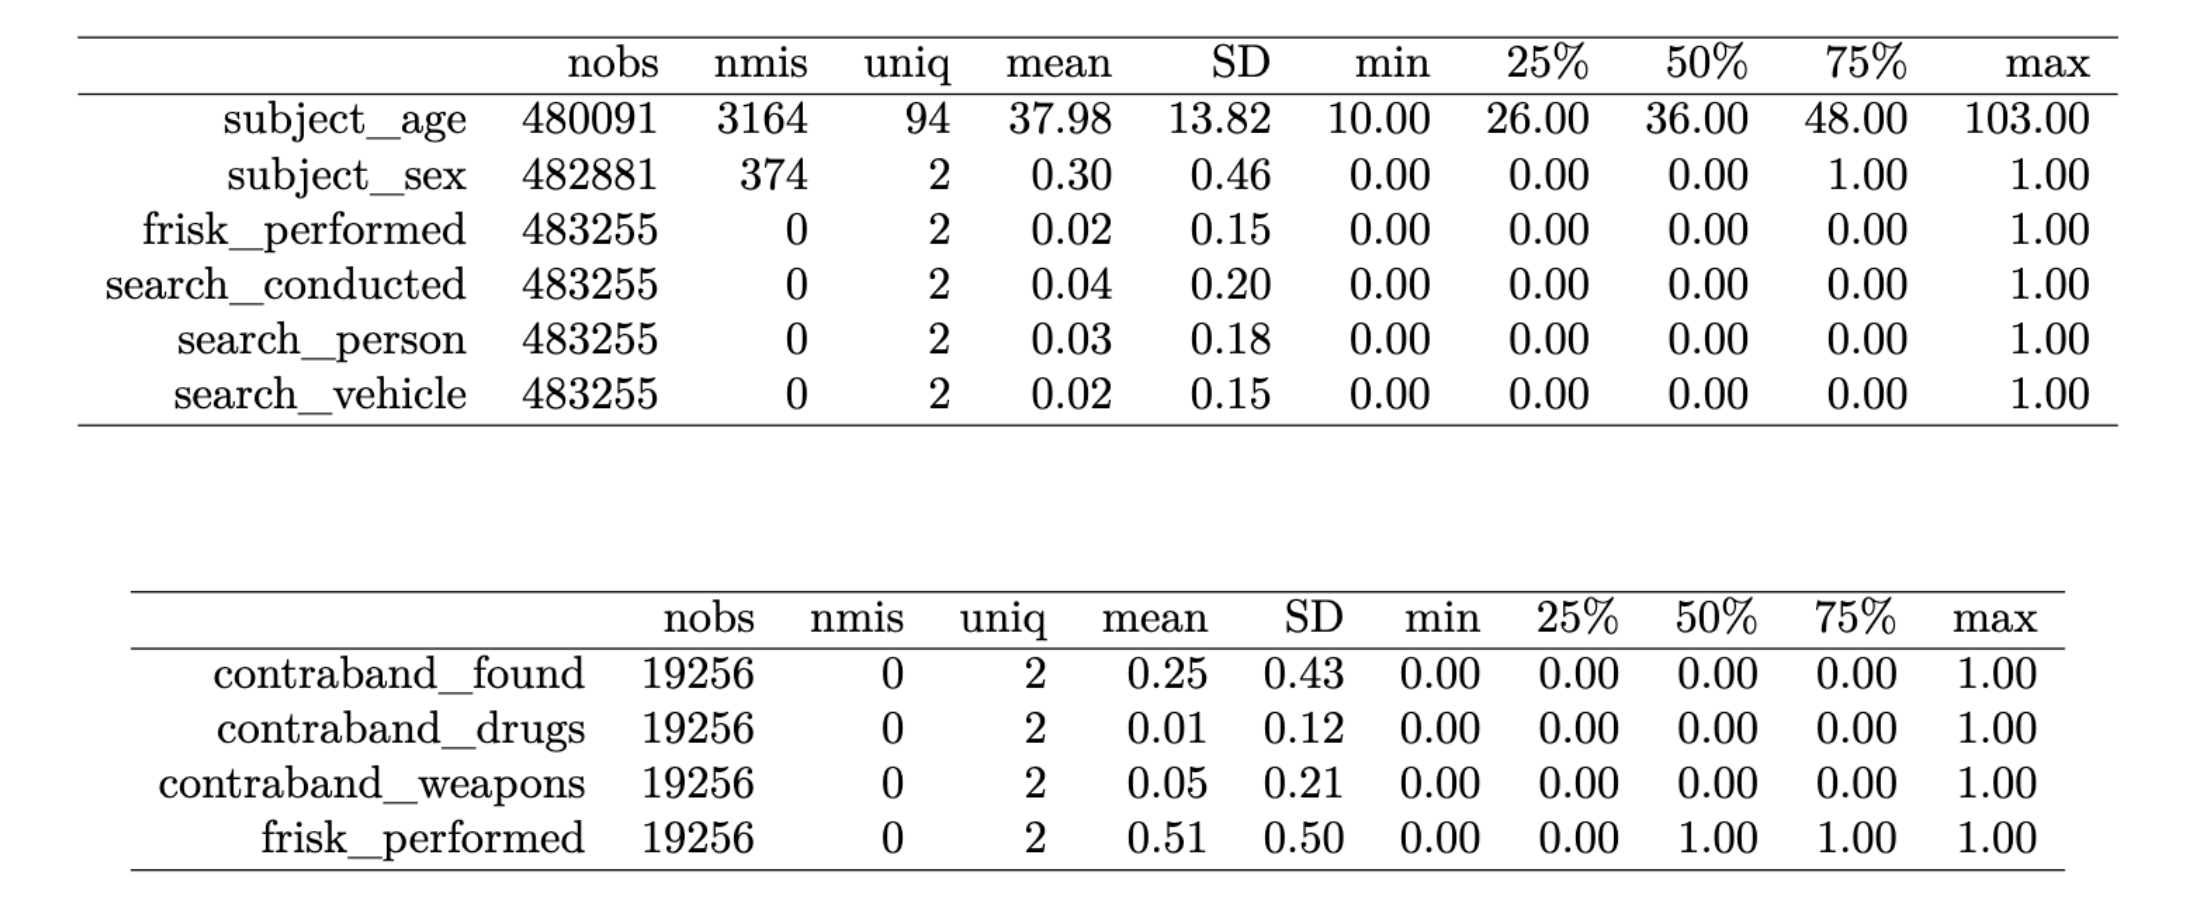
\includegraphics[width=10cm]{pic2.pdf}
\caption{Hit rates for individual officers} \label{fg:2}
\end{figure}

Figure \ref{fg:2} shows the hit rates for individual officers. An officer with an identical hit rate for white and minority subpopulations would be on the 45-degree line. Visually, it is difficult to determine a systematic trend, although it is clear that particular officers have hit rates that differ substantially by subpopulaton. It should be noted that the hit rate is highly variable with small sample sizes.\\ 

We proceed using a Bayesian hierarchical model. Under this model, we treat individual officers as belonging to a population and we seek to model both the hit rates of the officers and the variation of this population. This permits partial pooling, by which individual hit rates are biased towards the population average by an amount determined by the estimate of the population. For each officer, we consider three hit rates, one each for white, Black, and Hispanic subpopulations. We accomplish this by fitting separate Bayesian logistic mixed effects models for each race, each with a weakly informative Normal prior on the log-odds with mean $-1.3$ and standard deviation $1$.\\ 

Specifically, let $\theta_{jr}$ be the hit rate for for officer $j$ and race $r$, $y_{jr}$ be the number of hits, and $K_{jr}$ the number of frisks. In the following, because we fit separate models, we assume for example $r = black$ and drop the $r$ subscript. Assuming each officer’s searches are independent Bernoulli trials

$$ p(y_j|\theta_j) = \text{Binomial}(y_j|K_j,\theta_j) $$
We reparametrize the model in terms of the log-odds, $\alpha$:

$$ \alpha_j = \text{logit}(\theta_j)=\log\frac{\theta_j}{1-\theta_j} $$
We set a weakly informative prior centered at $\alpha_j = -1.3$, corresponding to $\theta_j\approx 0.2$. The model is therefore
$$ p(y_j|K_j, \alpha) = \text{Binomial}(y_j|K_j,\text{logit}^{-1}(\alpha_j)) $$

We proceed using \texttt{stan\_glmer} and the default prior on the covariance matrix. The result includes a posterior for each officer; we may transform from the log-odds back to hit rate to to obtain a posterior for the the hit rate for each officer. We model each race separately, and so obtain three posteriors for each officer. Table \ref{tb:8} shows the posteriors for the first several officers (rows) for each of the three races (columns).\\



\begin{table}
\centering
\begin{tabular}{|ccc|} 
\hline
2.5\%& 50\% &97.5\%\\
\hline
0.003& 0.055& 0.317\\
0.021& 0.095& 0.248\\
0.003& 0.056& 0.324\\
0.128& 0.523& 0.900\\
0.054& 0.188& 0.415\\
0.114& 0.380 &0.722\\
\hline
\end{tabular}
\begin{tabular}{|ccc|} 
\hline
2.5\%& 50\% &97.5\%\\
\hline
0.021 &0.198 &0.617\\
0.002 &0.033 &0.203\\
0.111 &0.242 &0.420\\
0.057 &0.521 &0.959\\
0.032 &0.332 &0.833\\
0.002 &0.040 &0.261\\
\hline
\end{tabular}
\begin{tabular}{|ccc|} 
\hline
2.5\%& 50\% &97.5\%\\
\hline
0.065 &0.214 &0.450\\
0.047 &0.162 &0.359\\
0.037 &0.174 &0.423\\
0.665 &0.874 &0.974\\
0.082 &0.268 &0.556\\
0.010 &0.071 &0.237\\
\hline
\end{tabular}
\caption{Posterior intervals for three races. From left to right: white, Black, Hispanic} \label{tb:8}
\end{table}


The effects of partial pooling are evident: the posterior medians are baised towards the population average. Practically, this means that observed hit rates equal to zero have posterior medians that are small but positive, and perfect (or near-perfect) observed hit rates have somewhat smaller posterior medians.


\begin{figure}[H]
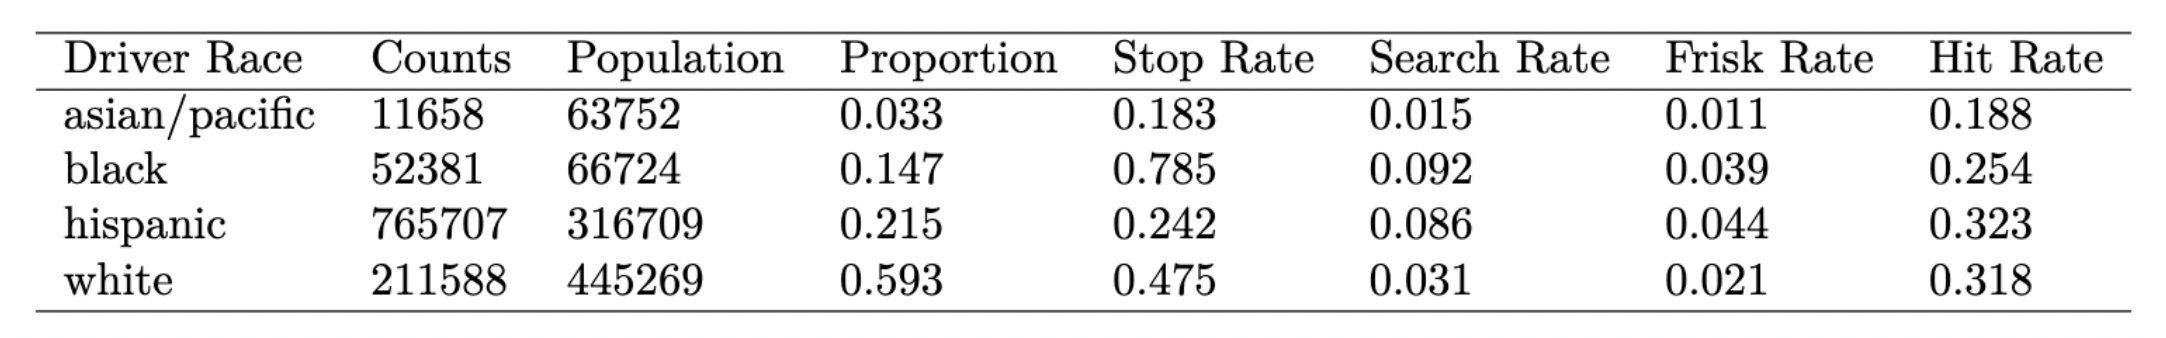
\includegraphics[width=\textwidth]{pic3.pdf}
\caption{Posterior medians for three races} \label{fg:3}
\end{figure}


Because part of this project is to “operationalize” fairness, we devised a measure by which the above posteriors can be converted into a rough “fairness score.” Because an officer that uses the same evidence threshold when deciding whether to frisk a subject regardless of race should have roughly equal hit rates for all three subpopulations, we reason that such an officer should have posterior medians that are close to each other for the three subpopulations. So, one can calculate a simple sum of squares statistic for each officer. Specifically, letting $m_{jr}$ be the posterior median for officer $j$ and race $r$, the sum of squares statistic $S_j$ is

$$ S_j =\sum_r( m_{jr}- \bar{m}_{j})^2 $$

where $\bar{m}_j$ is the average of the three medians. Of course, this measure disregards all other information that could be gleaned from the posterior; an alternative might calculate the overlap between the posterior densities. However, we think this measure is relatively easy to understand and implement.


\begin{table}
\centering
\begin{tabular}{l*{10}{c}} 
\hline
ID &obs.w& obs.b &obs.h& post.w& post.b &post.h &count.w &count.b& count.h\\
\hline
1504c3bc16 &1.000 &0.227 &0.143& 0.697& 0.215 &0.142 &2 &22 &7\\
3392a495a3 &0.400 &0.000 &0.545& 0.371& 0.046 &0.499 &10& 5 &11\\
50f70c6ecb &0.583 &0.000 &0.167& 0.549& 0.064 &0.162 &12& 3 &18\\
bab7c2acaf &0.833 &0.333 &0.750& 0.644& 0.247 &0.715 &7 &3 &20\\
dd9c1003d5 &0.556 &0.000 &0.250& 0.513& 0.043 &0.210 &9 &6 &4\\
\hline
\end{tabular}
\caption{Highest 5 scores} \label{tb:9}
\end{table}


\begin{figure}[H]
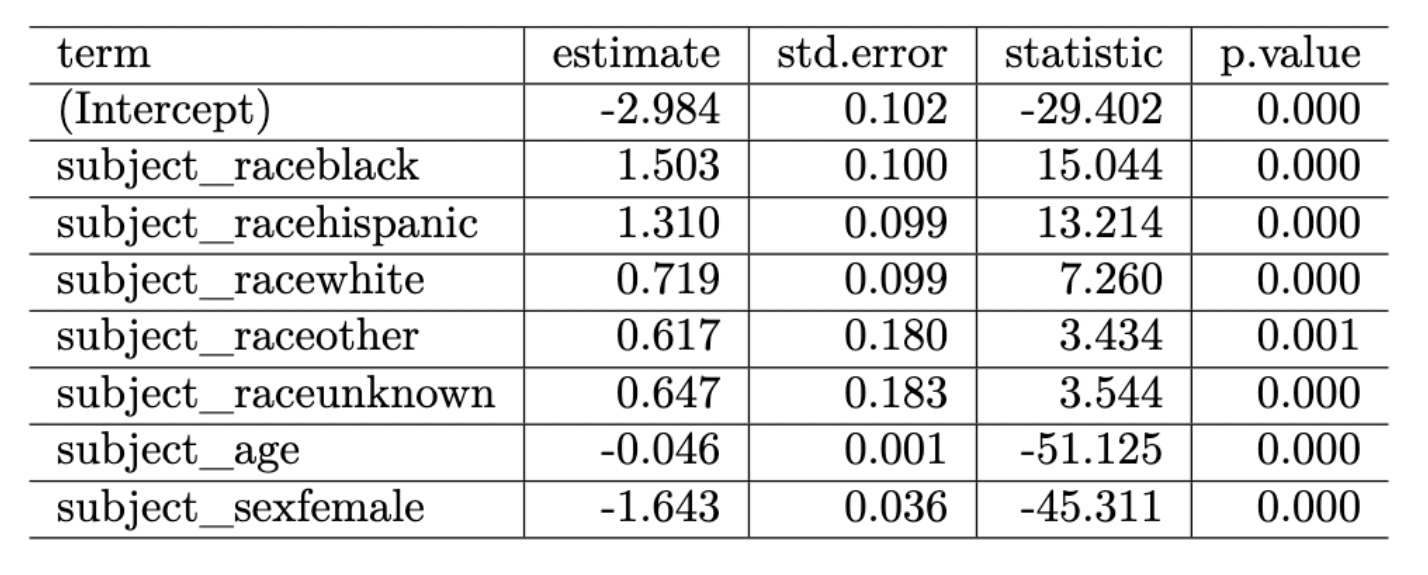
\includegraphics[width=\textwidth]{pic4.pdf}
\caption{Fairness scores for the officers under consideration. Lower scores indicate hit rates are more similar} \label{fg:4}
\end{figure}


\section{Conclusion}

In this study, we evaluate the fairness of traffic stops during the past two decades through three tests, namely benchmark test, outcome test and veil of darkness test. We found that the racial disparity in policing exists and is present in different scales spatially and temporarily. We also explore the causal confounding issues through logistic regression, finding that black and Hispanic people are more likely to be frisked and found with contraband items that are neither drugs or weapons.\\

Through the investigation of the hit rate via Bayesian hierarchical modeling, we obtained posteriors for the hit rate for each officer in a subset of the data. Using the medians for these posteriors, we devised a “fairness score,” a tool we believe could be used to identify officers with racially disparate patterns of traffic stops.

%%============================================================================%%
%%                                References                                  %%
%%============================================================================%%
\begin{thebibliography}{99}

\bibitem{1}
Grogger, Jeffrey, and Greg Ridgeway. "Testing for racial profiling in traffic stops from behind a veil of darkness." Journal of the American Statistical Association 101.475 (2006): 878-887.

\bibitem{2}
Carpenter, Bob, J. Gabry, and B. Goodrich. "Hierarchical partial pooling for repeated binary trials." (2016).

\bibitem{3}
Pierson, Emma, et al. "A large-scale analysis of racial disparities in police stops across the United States." Nature human behaviour 4.7 (2020): 736-745.

\bibitem{4}
Simoiu, Camelia, Sam Corbett-Davies, and Sharad Goel. "The problem of infra-marginality in outcome tests for discrimination." The Annals of Applied Statistics 11.3 (2017): 1193-1216.
\end{thebibliography}

\end{document}
%%%%%%%%%%%%%%%%%%%%%%%%%%%%%%%%%%%%%%%%%%%%%%%%%%%%%%%%%%%%%%%%%%
